%!TEX TS-program = xelatex

\documentclass[aspectratio=169]{beamer}

\newbool{russian}
%\booltrue{russian} % Uncomment if in Russian
\usepackage{graphicx}
\usepackage[dvipsnames]{xcolor}
\usepackage{tikz}
\usepackage{pgf}
\usetikzlibrary{positioning,fit,backgrounds,scopes,decorations.pathreplacing,shapes.geometric}
\usepackage{booktabs, multirow, tabularx}
\usepackage{mathspec}

\renewcommand\arraystretch{1.}

%%% Информация об авторе и выступлении
\title[GraphTyper]{GraphTyper: Neural Types Inference from Code Represented as Graph}
\author[authors]{
    \texorpdfstring{
        \begin{columns}
            \column{0.5\textwidth}
            \centering
            German Arutyunov \\ \smallskip \scriptsize \url{gaarutyunov@edu.hse.ru}\\\url{https://github.com/gaarutyunov/}
            \column{0.5\textwidth}
            \centering
            Sergey Avdoshin \\ \smallskip \scriptsize \url{savdoshin@hse.ru}\\\url{https://www.hse.ru/staff/avdoshin/}
        \end{columns}
    }{German Arutyunov, Sergey Avdoshin}
}
\institute{HSE University, 20, Myasnitskaya st., Moscow, Russia}
\date{\today}


\begin{document}

    \frame[plain]{\titlepage}

    \begin{frame}
        \frametitle{Introduction}
        \framesubtitle{Task definition, practical relevance and results}
        \begin{itemize}
            \item Task: Predicting type annotations in dynamically-typed languages (Python)
            \item Relevance:
            \begin{itemize}
                \item Errors due to wrong or absent type annotations
                \item Model flexibility for future work
            \end{itemize}
            \item Results:
            \begin{itemize}
                \item Masked transformer model that can be directly used on code represented as graph
            \end{itemize}
        \end{itemize}
    \end{frame}

    \begin{frame}
        \frametitle{Introduction}
        \framesubtitle{Structure}
        \begin{enumerate}
            \item Previous Work
            \item Proposed Solution
            \item Experiment Results and Ablation Analysis
            \item Final Model Quantitative Results
            \item Limitations and Workarounds
        \end{enumerate}
    \end{frame}

    \begin{frame}
        \frametitle{Previous Work}
        \framesubtitle{Main works}
        \begin{table}
            \centering
            \label{tab:main-works}
            \begin{tabularx}{\textwidth}{ccXc}
    \toprule
    Authors & Year & Title & Adoptions \\
    \midrule
    Allamanis et al. & 2020 & Typilus: Neural Type Hints & Dataset, Metrics \\
    Kim et al. & 2022 & Pure Transformers are Powerful Graph Learners & Model Architecture \\
    \bottomrule
\end{tabularx}
        \end{table}
    \end{frame}

    \begin{frame}
        \frametitle{Previous Work}
        \framesubtitle{Works for result comparison}
        \begin{table}
            \centering
            \label{tab:works-for-comparison}
            \begin{tabularx}{\textwidth}{ccXc}
    \toprule
    Authors & Year & Title & Model Name \\
    \midrule
    Allamanis et al. & 2020 & Typilus: Neural Type Hints & Typilus (GNN) \\
    Pradel et al. & 2020 & TypeWriter: neural type prediction with search-based validation & TypeWriter (RNN) \\
    Mir et al. & 2021 & Type4py: Deep similarity learning-based type inference for python & Type4py (RNN) \\
    Jesse et al. & 2021 & Learning type annotation: is big data enough? & TypeBERT (Transformer) \\
    Peng et al. & 2023 & Generative Type Inference for Python & TypeGen (Transformer) \\
    \bottomrule
\end{tabularx}
        \end{table}
    \end{frame}

    \begin{frame}
        \frametitle{Proposed Solution}
        \framesubtitle{Dataset}
        \begin{columns}
            \column{0.5\textwidth}
            \begin{itemize}
                \item 118,440 files with 5,997,459 symbols
                \item Top 10 types cover half of the dataset
                \item Only 158 types have over 100 annotations
                \item The majority are used fewer than 100 times each, forming 32\% of the dataset
            \end{itemize}
            \column{0.5\textwidth}
            \begin{figure}
                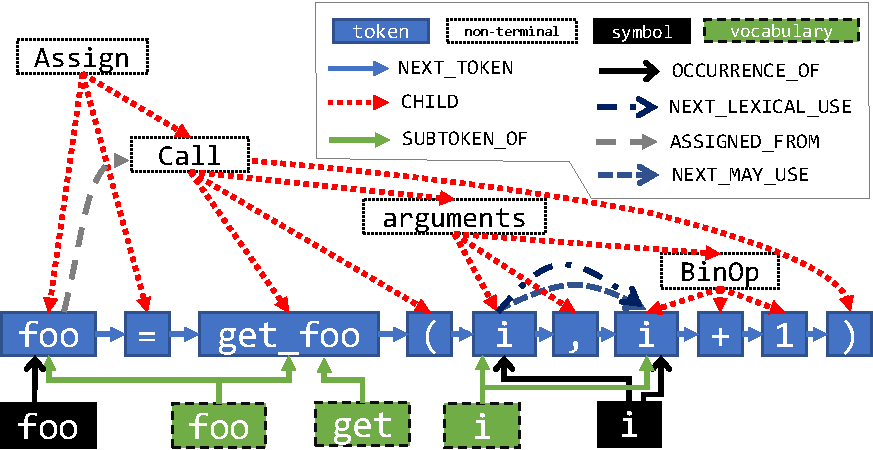
\includegraphics[width=\columnwidth]{figures/samplegraph.pdf}
                \caption{Sample graph for foo=get\_foo(i, i+1) showing different node categories and edge labels.}
                \label{fig:samplegraph}
            \end{figure}
        \end{columns}
    \end{frame}

    \begin{frame}
        \frametitle{Proposed Solution}
        \framesubtitle{Model architecture}
        \begin{figure}
            \resizebox{\textwidth}{!}{\begin{tikzpicture}[
code/.style={},
v1/.style={circle,fill=WildStrawberry,minimum size=16pt},
v2/.style={circle,fill=Peach,minimum size=16pt},
v3/.style={circle,fill=VioletRed,minimum size=16pt},
v4/.style={circle,fill=DarkOrchid,minimum size=16pt},
e1/.style={draw,line width=4pt,-,Emerald},
e2/.style={draw,line width=4pt,-,SpringGreen},
e3/.style={draw,line width=4pt,-,SpringGreen!50},
e4/.style={draw,line width=4pt,-,Emerald!50},
arrow/.style={draw,->,black},
dashed arrow/.style={dashed,draw,->,black},
identifier/.style={align=center,font=\small},
rounded/.style={rectangle,minimum size=16pt,rounded corners=4pt},
vi/.style={rounded,fill=RoyalBlue},
ei/.style={rounded,fill=RoyalBlue!50},
*|/.style={
    to path={
        (perpendicular cs: horizontal line through={(\tikztostart)},
        vertical line through={(\tikztotarget)})
        % is the same as (\tikztostart -| \tikztotarget)
        % but just to be safe: http://tex.stackexchange.com/a/29781/16595
        -- (\tikztotarget) \tikztonodes
    }
},
]

% Source code
\node[code,label={[font=\small]below:Source code}] (code) {
\includegraphics[width=30pt,keepaspectratio]{assets/py_code.png}};

% AST Graph
\node[v1,label=above:$V1$,right=40pt of code,yshift=-15pt] (v1) {};
\node[v2,label=above:$V2$,above right=20pt and 20pt of v1] (v2) {};
\node[v3,label=above:$V3$,right=40pt of v1] (v3) {};
\node[v4,label=above:$V4$,above right=20pt and 20pt of v3] (v4) {};

\path[e1] (v1) -- (v2);
\path[e2] (v2) -- (v4);
\path[e3] (v3) -- (v2);
\path[e4] (v4) -- (v3);

\node[fit=(v1) (v2) (v3) (v4),label={[font=\small]below:AST Graph}] (graph) {};

\path[arrow] (code) -- (graph);

% Identifiers
\node[identifier,above right=30pt and 12pt of v4] (ti) {Type\\Identifiers};

\node[vi,right=25pt of ti,label={[font=\small]below:[node]}] (v) {v};
\node[ei,right=10pt of v,label={[font=\small]below:[edge]}] (e) {e};

\node[below=10pt of ti,identifier] (ni) {Node\\Identifiers};

\node[v1,rounded,right=5pt of ni] (n1) {1};
\node[v2,rounded,right=5pt of n1] (n2) {2};
\node[v3,rounded,right=5pt of n2] (n3) {3};
\node[v4,rounded,right=5pt of n3] (n4) {4};

\path[draw,decorate,decoration={brace,mirror,amplitude=5pt,raise=2pt}] (n1.south) -- (n4.south) node[midway,below=5pt,font=\small] (orthnormal) {orthonormal};

    {[on background layer]
\node[fit=(ti) (ni) (v) (e) (n1) (n2) (n3) (n4) (orthnormal),fill=Gray!20,above right=-20pt and 10pt of v4,minimum size=60pt,rounded corners=4pt] (identifiers) {};
}

\path[dashed arrow] (graph) |- (identifiers);

\path[draw,->,black] (n4)+(15pt,0) -- +(35pt,0);
\path[draw,->,black] (e)+(33pt,0) -- +(53pt,0);

% V1

\node[v1,rounded,right=40pt of n4.north,yshift=0.5pt] (nt1-1) {1};
\node[v1,rounded,below=1pt of nt1-1] (nt1-2) {1};

    {[on background layer]
\node[fit=(nt1-1) (nt1-2),rounded corners=4pt,rectangle,draw=black] (nt1) {};
}

\node[vi,above=10pt of nt1-1] (vi-1) {v};

\node[v1,below=27pt of nt1-1] (v1-1) {};

\path[draw,->,black] (graph.center)+(35pt,-5pt) -- (332pt,-5pt) node[midway,below=5pt,font=\small] (mask) {Randomly masked type annotations};

    {[on background layer]
\path[draw,->,black] (v1-1) -- +(0,95pt);
}

% E1

\node[v1,rounded,right=10pt of nt1-1] (nt2-1) {1};
\node[v2,rounded,below=1pt of nt2-1] (nt2-2) {2};

    {[on background layer]
\node[fit=(nt2-1) (nt2-2),rounded corners=4pt,rectangle,draw=black] (nt2) {};
}

\node[ei,above=10pt of nt2-1] (ei-1) {e};

\node[below=27pt of nt2-1,opacity=0.0,minimum size=16pt,rectangle] (e1-1-tmp) {};
\node[fill=Emerald,below=27pt of nt2-1,node distance=10pt,minimum width=4pt,minimum height=16pt,rectangle,inner sep=0,rotate around={135:(e1-1-tmp.center)}] (e1-1) {};

    {[on background layer]
\path[draw,->,black] (e1-1) -- +(0,95pt);
}

% V2

\node[v2,rounded,right=10pt of nt2-1] (nt3-1) {2};
\node[v2,rounded,below=1pt of nt3-1] (nt3-2) {2};

    {[on background layer]
\node[fit=(nt3-1) (nt3-2),rounded corners=4pt,rectangle,draw=black] (nt3) {};
}

\node[vi,above=10pt of nt3-1] (vi-2) {v};

\node[v2,semicircle,minimum size=8pt,below=30.5pt of nt3-1,node distance=10pt] (v2-1) {};

    {[on background layer]
\path[draw,->,black] (v2-1) -- +(0,95pt);
}

% E2

\node[v2,rounded,right=10pt of nt3-1] (nt4-1) {2};
\node[v3,rounded,below=1pt of nt4-1] (nt4-2) {3};

    {[on background layer]
\node[fit=(nt4-1) (nt4-2),rounded corners=4pt,rectangle,draw=black] (nt4) {};
}

\node[ei,above=10pt of nt4-1] (ei-2) {e};

\node[below=27pt of nt4-1,opacity=0.0,minimum size=16pt,rectangle] (e2-1-tmp) {};
\node[fill=SpringGreen!50,below=27pt of nt4-1,node distance=10pt,minimum width=4pt,minimum height=16pt,rectangle,inner sep=0,rotate around={45:(e2-1-tmp.center)}] (e2-1) {};

    {[on background layer]
\path[draw,->,black] (e2-1) -- +(0,95pt);
}

% V3

\node[v3,rounded,right=10pt of nt4-1] (nt5-1) {3};
\node[v3,rounded,below=1pt of nt5-1] (nt5-2) {3};

    {[on background layer]
\node[fit=(nt5-1) (nt5-2),rounded corners=4pt,rectangle,draw=black] (nt5) {};
}

\node[vi,above=10pt of nt5-1] (vi-3) {v};

\node[v3,semicircle,minimum size=8pt,below=30.5pt of nt5-1,node distance=10pt] (v3-1) {};

    {[on background layer]
\path[draw,->,black] (v3-1) -- +(0,95pt);
}

% E3

\node[v3,rounded,right=10pt of nt5-1] (nt6-1) {3};
\node[v4,rounded,below=1pt of nt6-1] (nt6-2) {4};

    {[on background layer]
\node[fit=(nt6-1) (nt6-2),rounded corners=4pt,rectangle,draw=black] (nt6) {};
}

\node[ei,above=10pt of nt6-1] (ei-3) {e};

\node[below=27pt of nt6-1,opacity=0.0,minimum size=16pt,rectangle] (e3-1-tmp) {};
\node[fill=Emerald!50,below=27pt of nt6-1,node distance=10pt,minimum width=4pt,minimum height=16pt,rectangle,inner sep=0,rotate around={135:(e3-1-tmp.center)}] (e3-1) {};

    {[on background layer]
\path[draw,->,black] (e3-1) -- +(0,95pt);
}

% V4

\node[v4,rounded,right=10pt of nt6-1] (nt7-1) {4};
\node[v4,rounded,below=1pt of nt7-1] (nt7-2) {4};

    {[on background layer]
\node[fit=(nt7-1) (nt7-2),rounded corners=4pt,rectangle,draw=black] (nt7) {};
}

\node[vi,above=10pt of nt7-1] (vi-4) {v};

\node[v4,below=27pt of nt7-1,node distance=10pt] (v4-1) {};

    {[on background layer]
\path[draw,->,black] (v4-1) -- +(0,95pt);
}

% E3

\node[v4,rounded,right=10pt of nt7-1] (nt8-1) {4};
\node[v2,rounded,below=1pt of nt8-1] (nt8-2) {2};

    {[on background layer]
\node[fit=(nt8-1) (nt8-2),rounded corners=4pt,rectangle,draw=black] (nt8) {};
}

\node[ei,above=10pt of nt8-1] (ei-4) {e};

\node[below=27pt of nt8-1,opacity=0.0,minimum size=16pt,rectangle] (e4-1-tmp) {};
\node[fill=SpringGreen,below=27pt of nt8-1,node distance=10pt,minimum width=4pt,minimum height=16pt,rectangle,inner sep=0,rotate around={90:(e4-1-tmp.center)}] (e4-1) {};

    {[on background layer]
\path[draw,->,black] (e4-1) -- +(0,95pt);
}


\path (v2-1) -- (e3-1) node[identifier,midway,below=12pt] (embeddings) {Node and Edge Tokens\\with Token-wise Embedding};

% Transformer

\node[fit=(nt1-1) (nt1-2) (nt2-1) (nt2-2) (nt3-1) (nt3-2) (nt4-1) (nt4-2) (nt5-1) (nt5-2) (nt6-1) (nt6-2) (nt7-1) (nt7-2) (nt8-1) (nt8-2),fill=Gray!20,rounded,draw,label=center:Transformer Encoder + MLP,above=20pt of vi-1,anchor=south west,xshift=-12pt] (transformer) {};

% Prediction

\node[v2,above=80pt of vi-2] (vp-2) {};
\node[v3,above=80pt of vi-3] (vp-3) {};

\path[draw,->,*|,black,shorten >=2pt] (transformer.north) to (vp-2);

\path[draw,->,*|,black,shorten >=2pt] (transformer.north) to (vp-3);

\path (vp-2) -- (vp-3) node[identifier,midway,above=12pt] (embeddings) {Type annotation predictions};


\end{tikzpicture}}
            \label{fig:model}
        \end{figure}
    \end{frame}

    \begin{frame}
        \frametitle{Proposed Solution}
        \framesubtitle{Metrics}

        To test the model, we use two metrics from the Typilus paper:

        \begin{itemize}
            \item Exact Match: Predicted and ground truth types match exactly.
            \item Match up to Parametric Type: Exact match when ignoring all type parameters.
        \end{itemize}
    \end{frame}

    \begin{frame}
        \frametitle{Experiment Results and Ablation Analysis}
        \framesubtitle{Hypothesis}
        \begin{enumerate}
            \item Validating the necessity of node and type identifiers that encode graph structure
            \item Using the model without node type annotations
            \item Increasing the number of parameters
            \item Testing different context length
            \item Testing different Transformer architectures
        \end{enumerate}
    \end{frame}

    \begin{frame}
        \frametitle{Experiment Results and Ablation Analysis}
        \framesubtitle{Results Discussion}
        \begin{table}
            \centering
            \label{tab:ablation}
            \begin{tabular}{lrrrrrr}
\toprule
Top-n & \multicolumn{2}{r}{Top-1} & \multicolumn{2}{r}{Top-3} & \multicolumn{2}{r}{Top-5} \\
Metric & EM & UTPT & EM & UTPT & EM & UTPT \\
\midrule
Plane Transformer & 10.15 & 19.46 & 15.06 & 29.40 & 16.81 & 37.91 \\
+ Node \& Type Identifiers & 30.88 & 36.55 & 40.33 & 50.37 & 42.82 & 56.01 \\
+ Type Annotations & 33.36 & \bfseries 42.28 & 41.71 & 52.90 & 43.62 & 57.00 \\
+ Decoder (Autoencoder) & 15.90 & 16.65 & 28.26 & 32.81 & 44.17 & 56.33 \\
or Longer Context & \bfseries 38.49 & 39.80 & \bfseries 53.14 & \bfseries 57.41 & \bfseries 58.80 & \bfseries 67.38 \\
or More Parameters & 29.39 & 31.82 & 44.85 & 49.72 & 49.74 & 56.14 \\
\bottomrule
\end{tabular}


        \end{table}
    \end{frame}

    \begin{frame}
        \frametitle{Final Model Quantitative Results}
        \framesubtitle{Comparison with previous work}
        \begin{table}
            \centering
            \label{tab:results}
            \begin{tabular}{lrrrrrr}
\toprule
Top-n & \multicolumn{2}{r}{Top-1} & \multicolumn{2}{r}{Top-3} & \multicolumn{2}{r}{Top-5} \\
Metric & EM & UTPT & EM & UTPT & EM & UTPT \\
\midrule
GraphTyper & 34.71 & 36.43 & 45.47 & 55.02 & 50.70 & 64.58 \\
\cline{1-7}
TypeBERT & 45.40 & 48.10 & 51.40 & 53.50 & 54.10 & 56.50 \\
TypeWriter & 56.10 & 58.30 & 63.70 & 67.30 & 65.90 & 70.40 \\
Typilus & 66.10 & 74.20 & 71.60 & 79.80 & 72.70 & 80.90 \\
Type4Py & 75.80 & 80.60 & 78.10 & 83.80 & 78.70 & 84.70 \\
TypeGen & \bfseries 79.20 & \bfseries 87.30 & \bfseries 85.60 & \bfseries 91.00 & \bfseries 87.00 & \bfseries 91.70 \\
\bottomrule
\end{tabular}


        \end{table}
    \end{frame}

    \begin{frame}
        \frametitle{Limitations and Workarounds}
        \framesubtitle{Considerations for future work}
        \begin{itemize}
            \item Type Vocabulary Size
            \item Absence of Natural Language Information
        \end{itemize}
        \begin{figure}
            \centering
            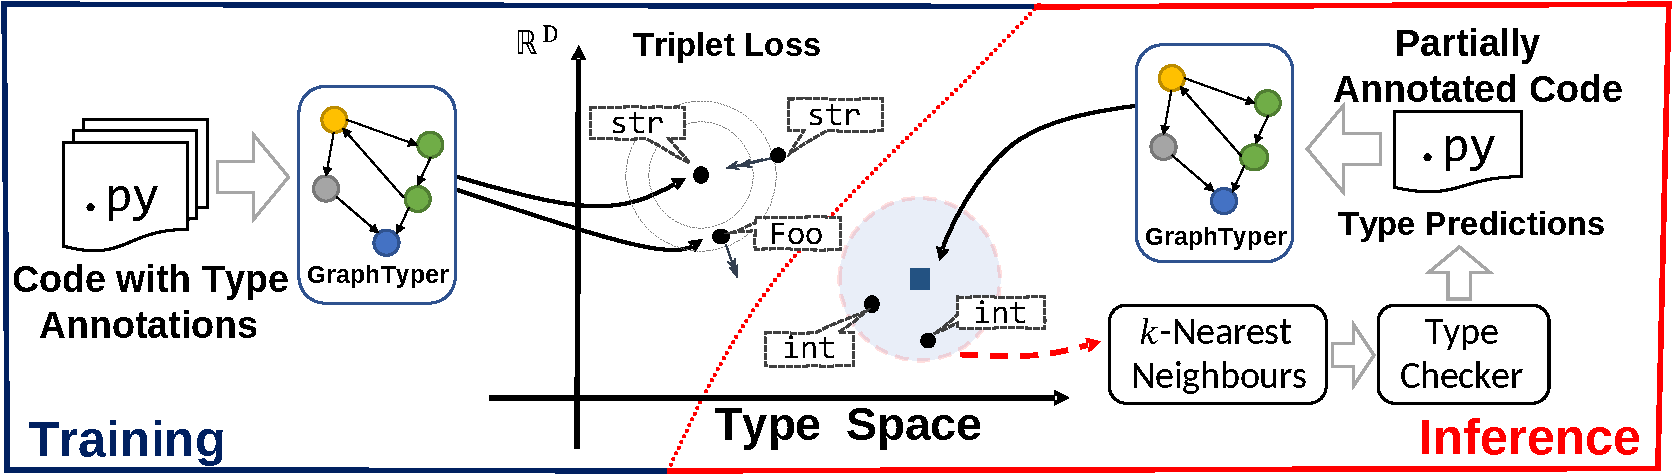
\includegraphics[width=\textwidth]{figures/dsl.pdf}
            \caption{Solution to the problem using Deep Similarity Learning.}
            \label{fig:dsl}
        \end{figure}
    \end{frame}

    \begin{frame}
        \frametitle{Conclusion}
        \begin{itemize}
            \item Main accomplishment:
            \begin{itemize}
                \item A universal Transformer model that can be applied on code represented as graph
            \end{itemize}
            \item Future Work:
            \begin{itemize}
                \item Universal code graph representation
                \item Detecting duplicates
                \item Code and docstring generation
                \item Vulnerability and error detection
                \item Refactoring
            \end{itemize}
        \end{itemize}
    \end{frame}

    \begin{frame}
        \frametitle{Acknolegements}
        This research was supported in part through computational resources of HPC facilities at HSE University~\footnote{
            P. S. Kostenetskiy, R. A. Chulkevich, and V. I. Kozyrev. “HPC Resources of the Higher School of Economics.” In: Journal of Physics: Conference Series 1740.1 (Jan. 2021)
        }
    \end{frame}

\end{document}